
\renewcommand{\EntradaBibtex}{DetecciónAlimentosEnAlbercas_SistemasInteligentes_UPV_2024}

\begin{frame}{\citetitle{\EntradaBibtex}$^*$ (1)}
\begin{block}{Motivación} 
Se requiere una herramienta para monitorear de manera remota a un grupo de usuarios de una alberca privada
\begin{itemize}
\item Se generardos dos conjuntos de entrenamiento: 
\begin{itemize}
\item Uno que incluye imágenes de albercas
\item Uno que incluye imágenes de personas consumiendo alimentos
\end{itemize}
\item Se entrenan los modelos por separado y posteriormente se combinan para generar la clasificación de salida. Específicamente se emplea el modelo YOLO (You only look once) v5 para detectar las personas con alimentos. 
\end{itemize}
\end{block} 
\footfullcite*{\EntradaBibtex}
\end{frame}


\begin{frame}{\citetitle{\EntradaBibtex} (2)}
%\begin{block}{Pantallas Principales} 

\begin{columns}
% Column 1
\column{.5\linewidth}

\begin{center}
	\begin{tabular}{cc}
		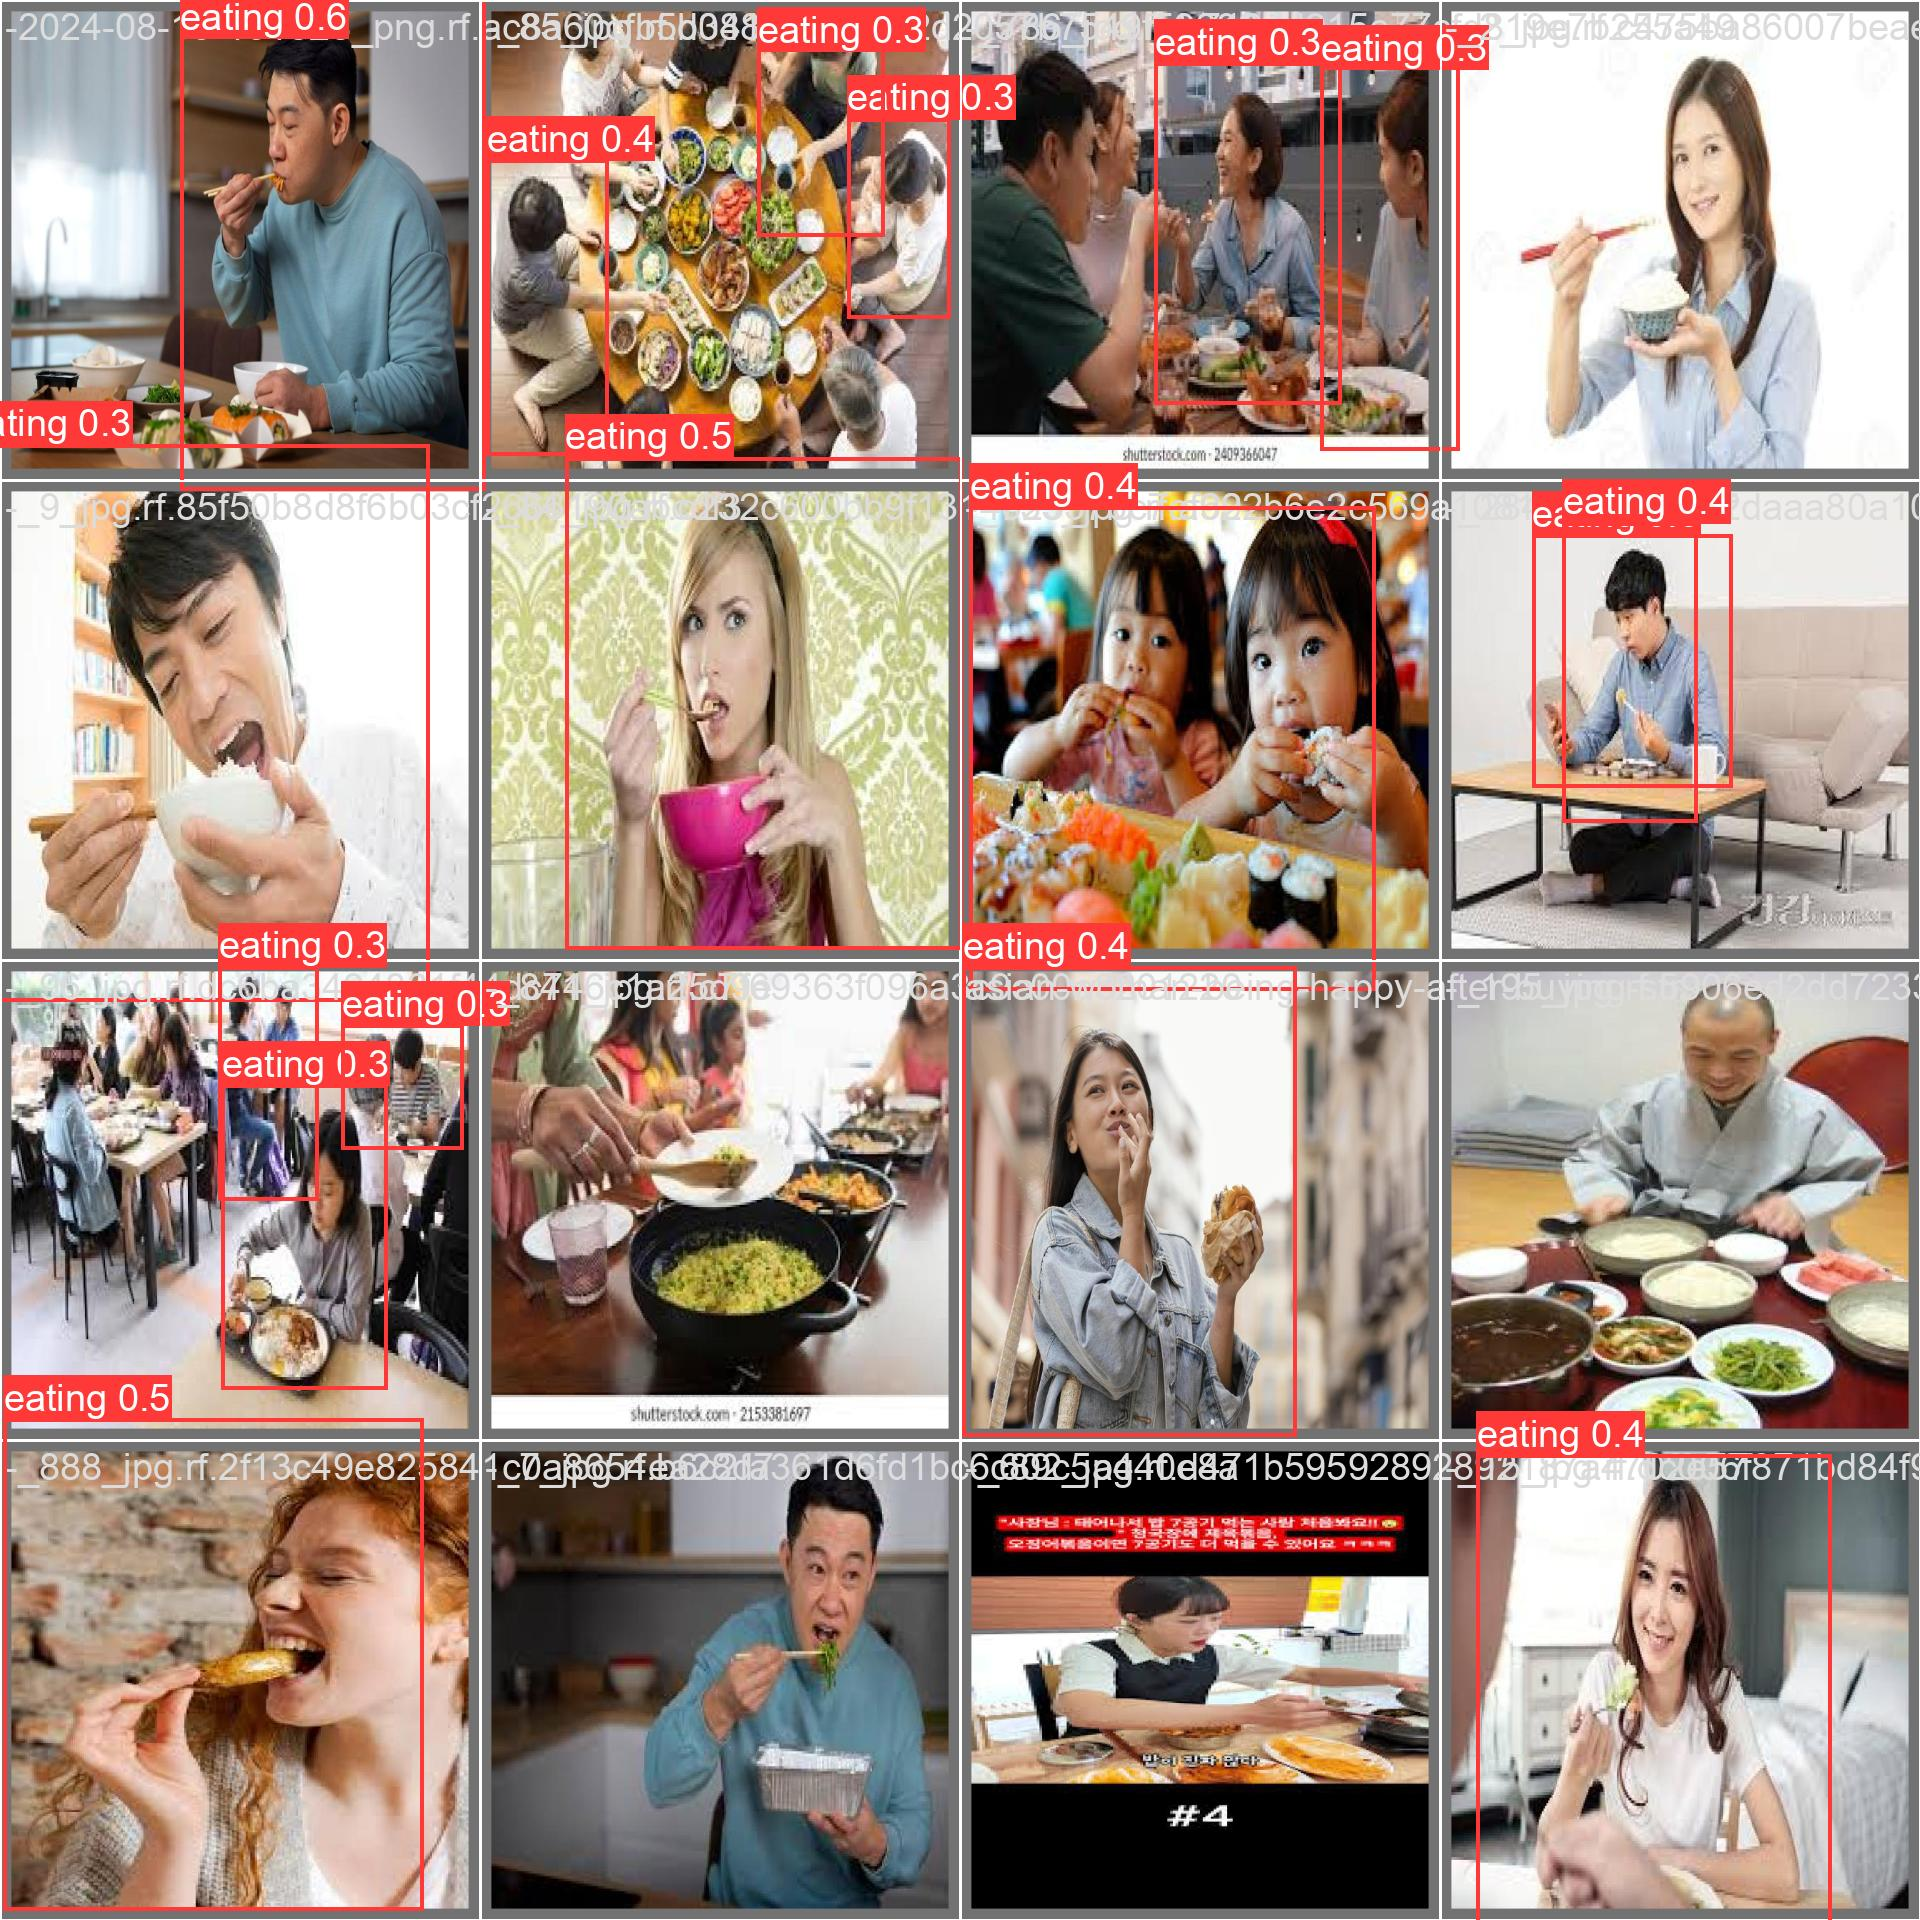
\includegraphics[width=0.48\linewidth]{2024_DeteccionAlimentosAlbercas/figs/val_batch0_pred.jpg} &
		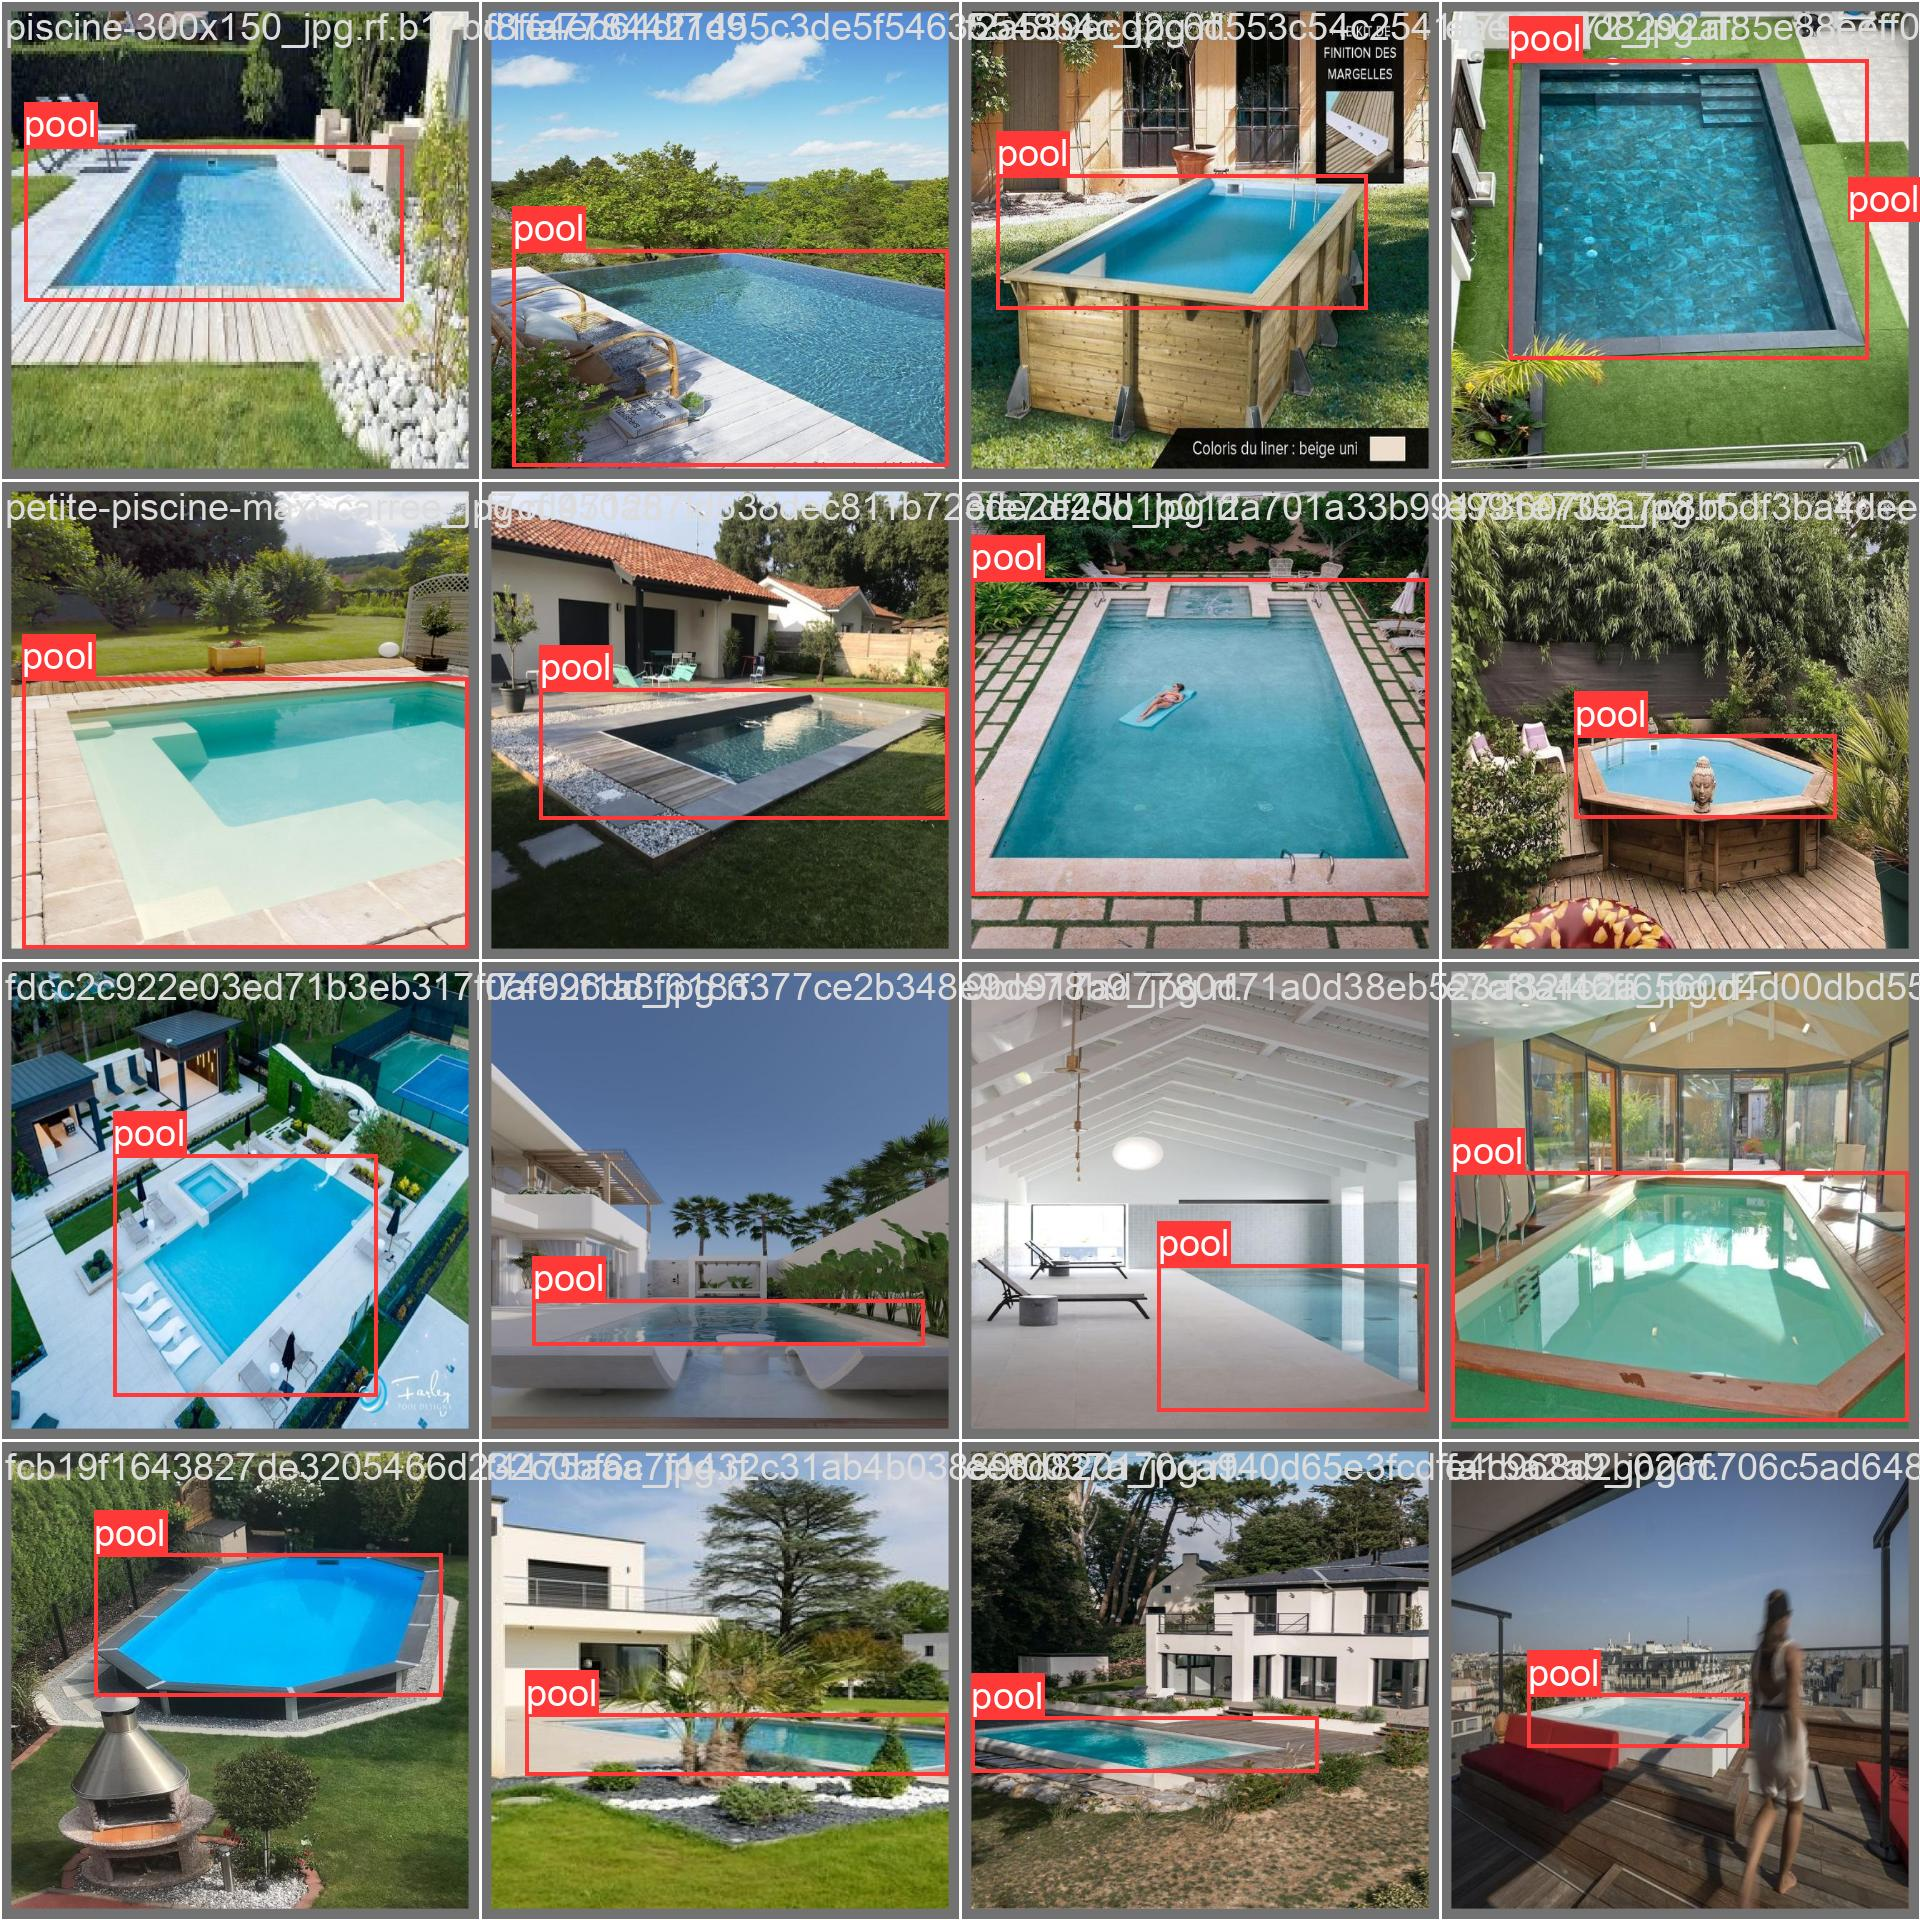
\includegraphics[width=0.48\linewidth]{2024_DeteccionAlimentosAlbercas/figs/val_batch1_labels.jpg} \\
	\end{tabular}
\end{center}

\column{.5\linewidth}
\begin{center}
	\begin{tabular}{cccc}
		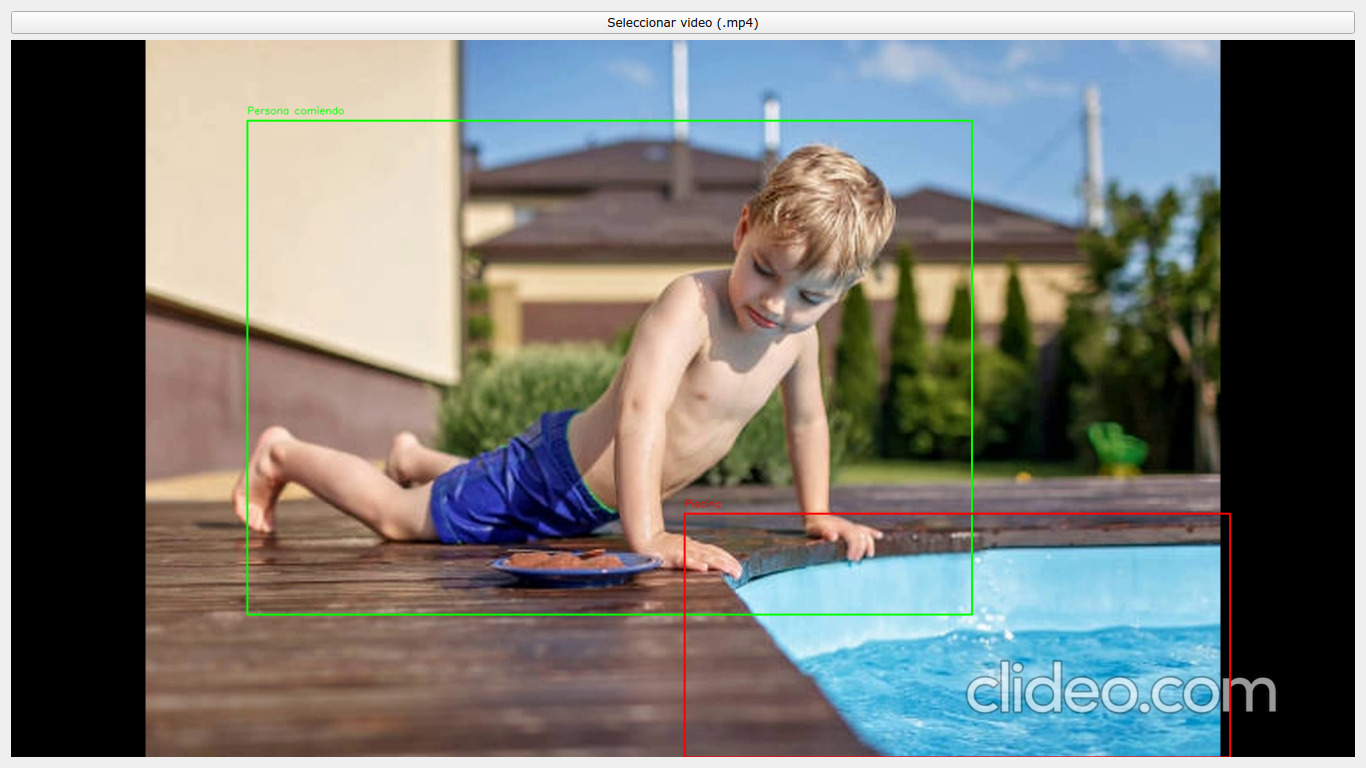
\includegraphics[width=0.48\linewidth]{2024_DeteccionAlimentosAlbercas/figs/im2.jpg} &
 		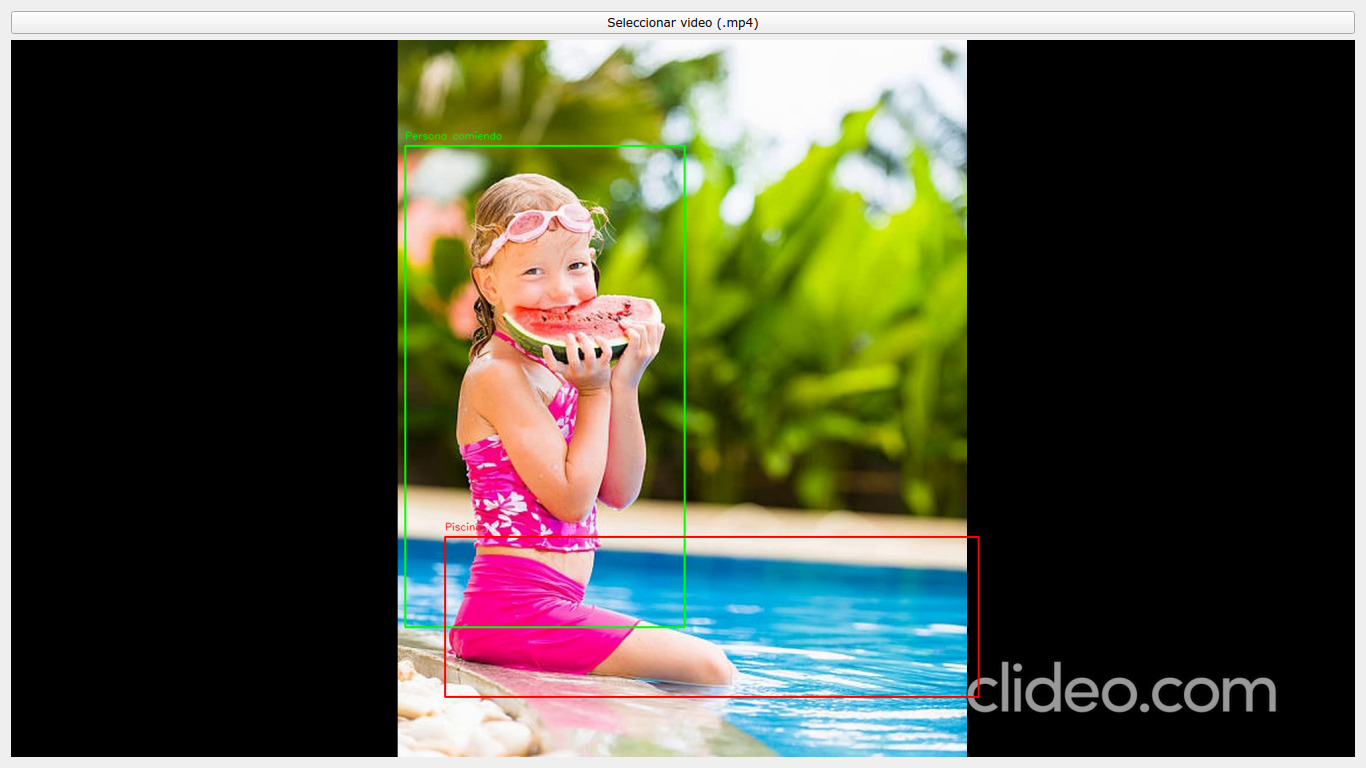
\includegraphics[width=0.48\linewidth]{2024_DeteccionAlimentosAlbercas/figs/im3.jpg} \\
		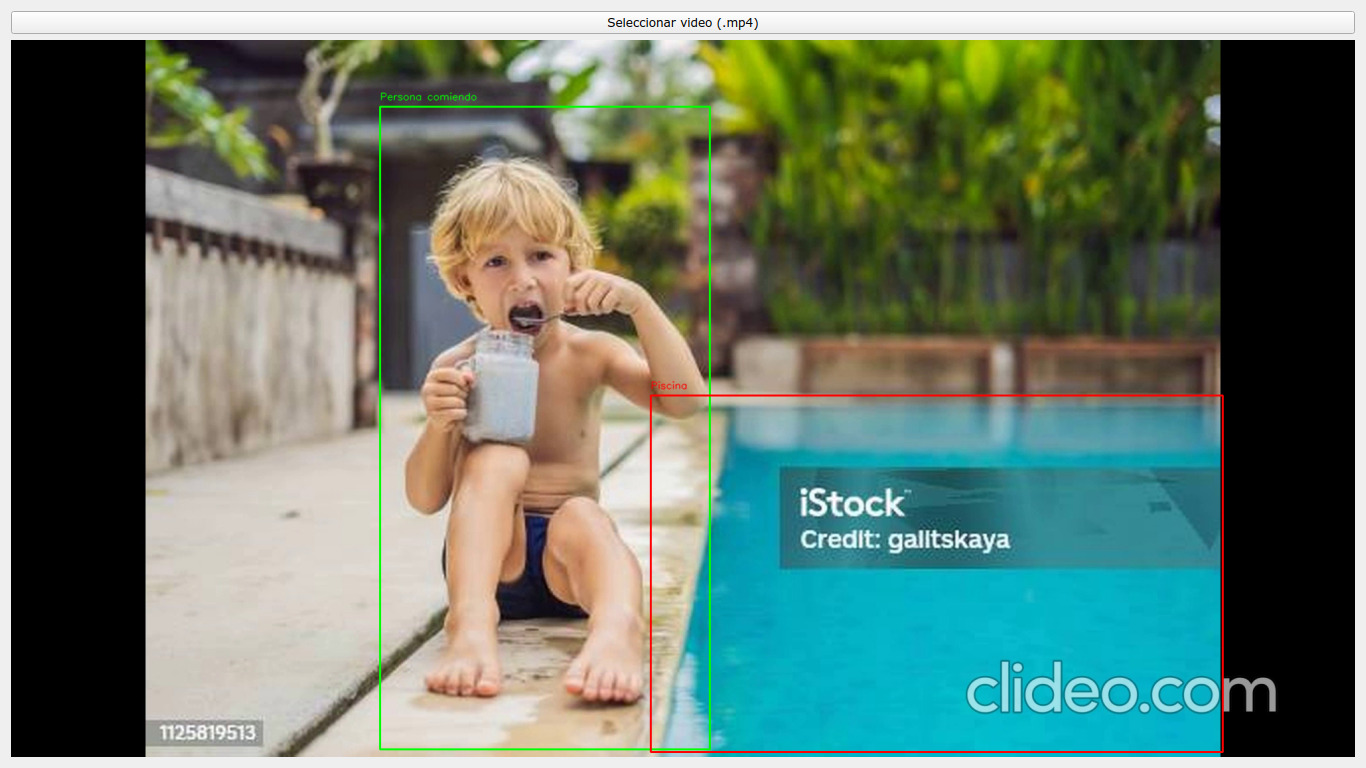
\includegraphics[width=0.48\linewidth]{2024_DeteccionAlimentosAlbercas/figs/im4.jpg} &
 		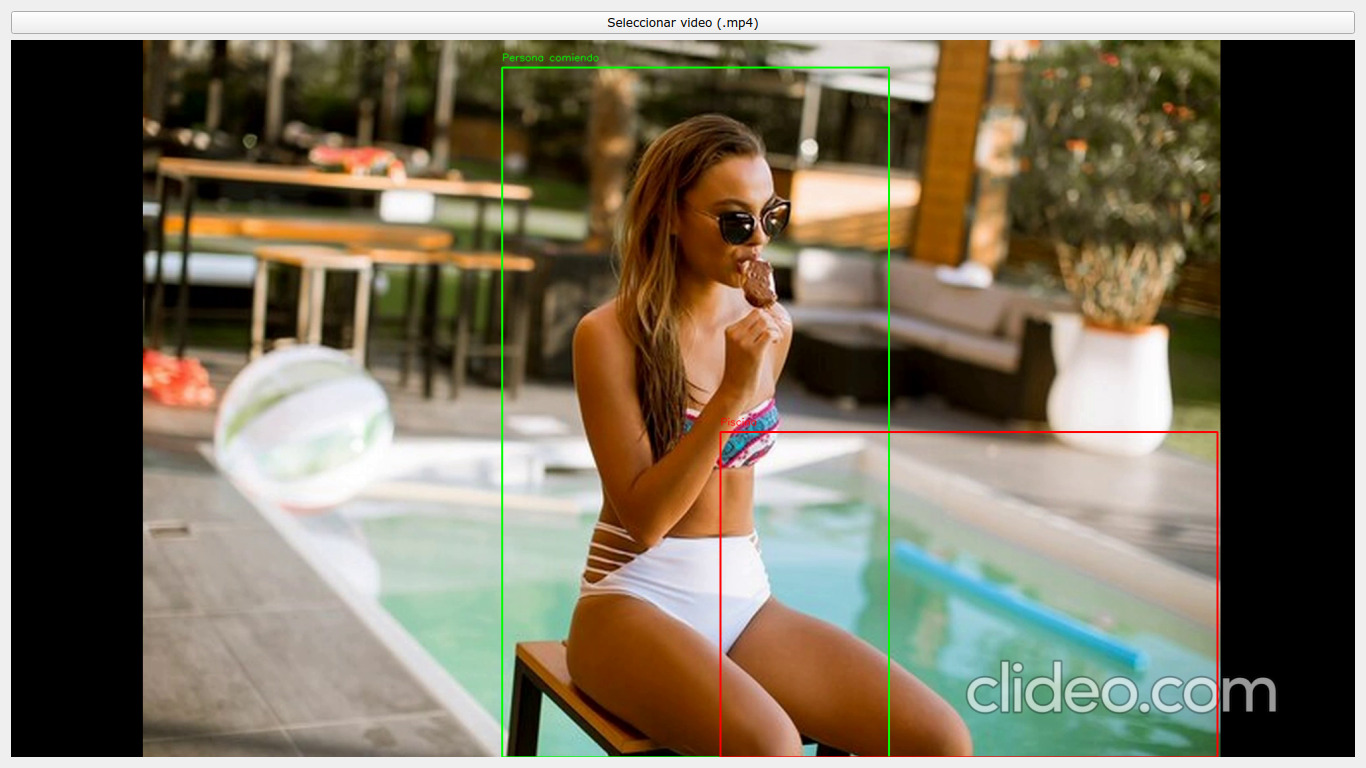
\includegraphics[width=0.48\linewidth]{2024_DeteccionAlimentosAlbercas/figs/im5.jpg} \\
	\end{tabular}
\end{center}


\end{columns}
\end{frame}





%/media/marco/Master/00_0A0RespadoLaptopHP_2024/Escritorio/00_DiapositivasProyectos/2024_PaseDeListaCodigoQR/figs/2.jpg
%/media/marco/Master/00_0A0RespadoLaptopHP_2024/Escritorio/00_DiapositivasProyectos/2024_PaseDeListaCodigoQR/figs/3.jpg
%/media/marco/Master/00_0A0RespadoLaptopHP_2024/Escritorio/00_DiapositivasProyectos/2024_PaseDeListaCodigoQR/figs/4.jpg


